This section contains the results for the SSP5-8.5, the gradual SAI and the rapid cooling SAI experiments, focusing on the atmospheric dynamics of the lower stratosphere.

\subsection{Potential temperature and Zonal Wind Anomaly}
The zonal mean potential temperature and potential temperature anomalies for Control, SAI 2020 and SAI 2080 are shown in Figures \ref{fig:th_U_zmdiff_ann} (annual mean), \ref{fig:th_U_zmdiff_JJA} (JJA) and \ref{fig:th_U_zmdiff_DJF} (DJF). The countours indicate the zonal mean zonal wind and zonal mean zonal wind anomalies. 

In Control we see the potential temperature anomaly signature of increased greenhouse gases, with warming at the surface and the troposphere, extending to the lower stratosphere and cooling in the upper stratosphere. In both SAI periods the potential temperature increases where SAI is deployed in the lower stratosphere, with the surface and troposphere showing no significant change. The anomaly in SAI 2020 is about 2.5°C larger than SAI 2080. In both SAI experiments the upper stratosphere shows the potential temperature decrease from greenhouse gases also observed in Control. 

The seasonal mean potential temperature anomalies show a larger increase in the summer over the Antarctic. In winter the latitudinal potential temperature gradient is larger, because the Antarctic receives no solar radiation during the polar night. 

The zonal mean zonal wind anomalies show that the most drastic changes in atmospheric dynamics occur in winter (JJA), thus we will focus on this season in our analysis of the lower stratosphere.

In Figure \ref{fig:th_U_zmdiff_JJA} the zonal mean of the zonal component of the thermal wind is shown, together with the observed zonal mean zonal wind in red countours. The observed wind and thermal wind show very similar patterns, with the observed wind consistently lower than the calculated thermal due to friction effects. The largest changes occur in the upper stratosphere, affecting the polar night jet, this will be discussed in section \ref{upperstrat}. 


\begin{figure}[H]
	\centering
	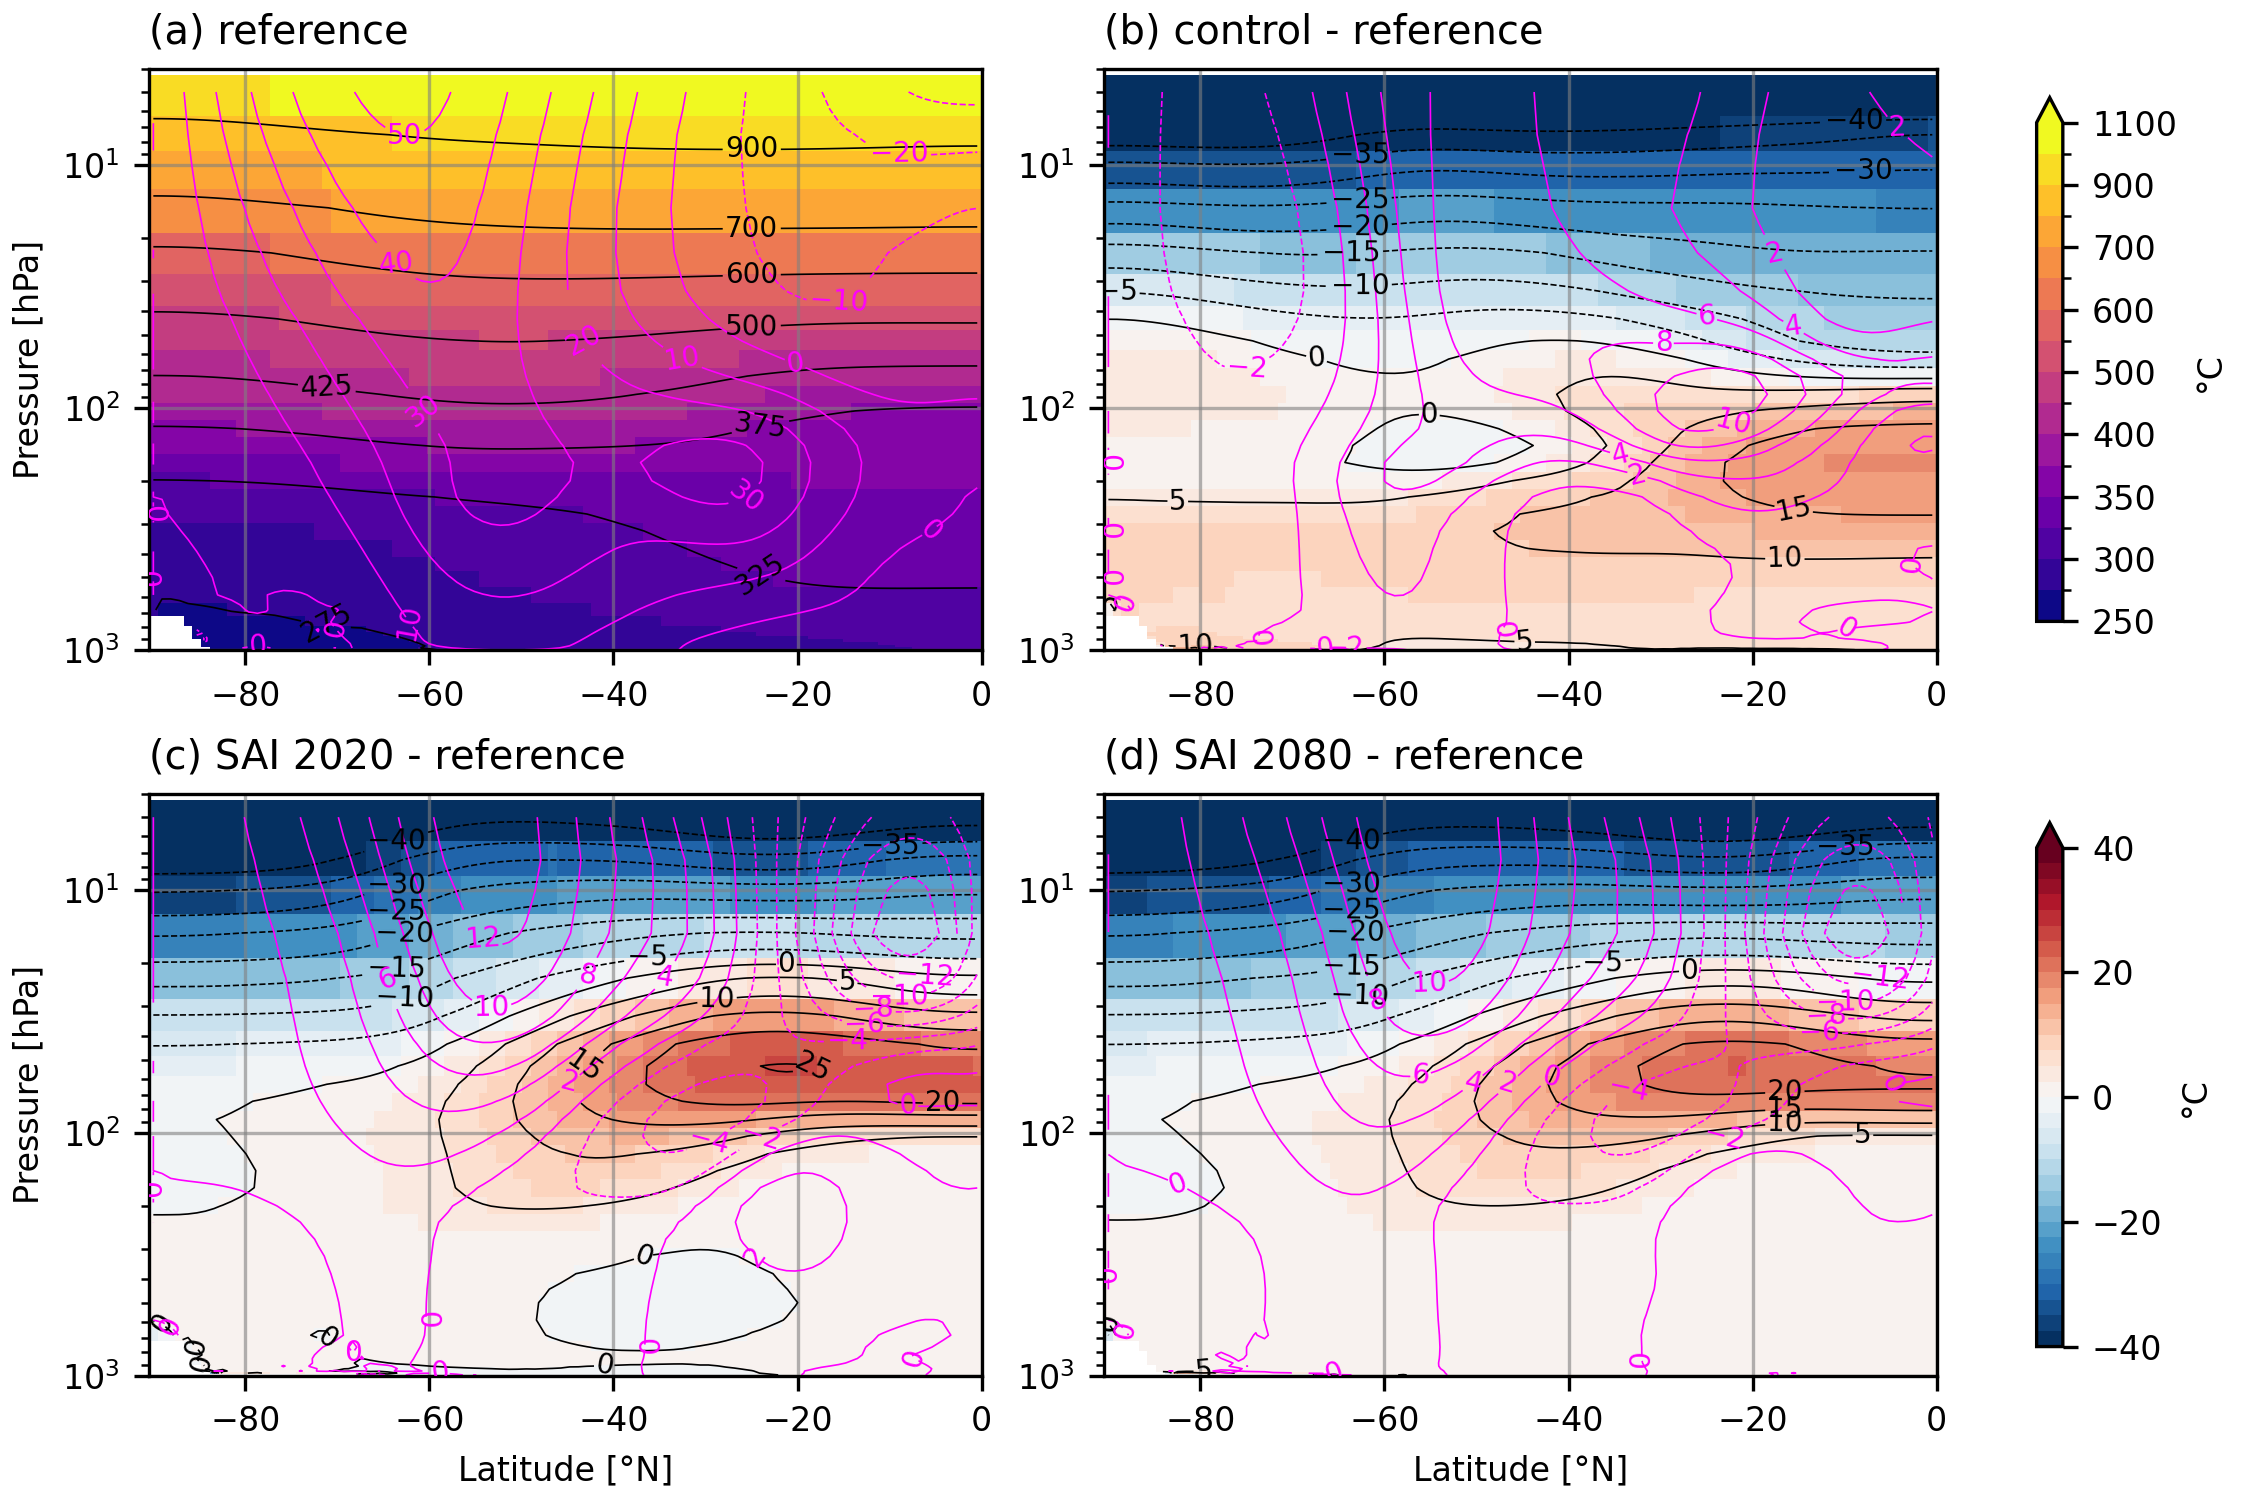
\includegraphics[width=0.95\linewidth]{images/th_U_zmdiff_ann.png}
	\caption{Annual mean zonal mean potential temperature (shading and black contours) and zonal mean zonal wind (magenta contours) for (a): Reference; (b-d): Control, SAI 2020 and SAI 2080 anomaly compared to Reference.}
	\label{fig:th_U_zmdiff_ann}
\end{figure}

\begin{figure}[H]
	\centering
	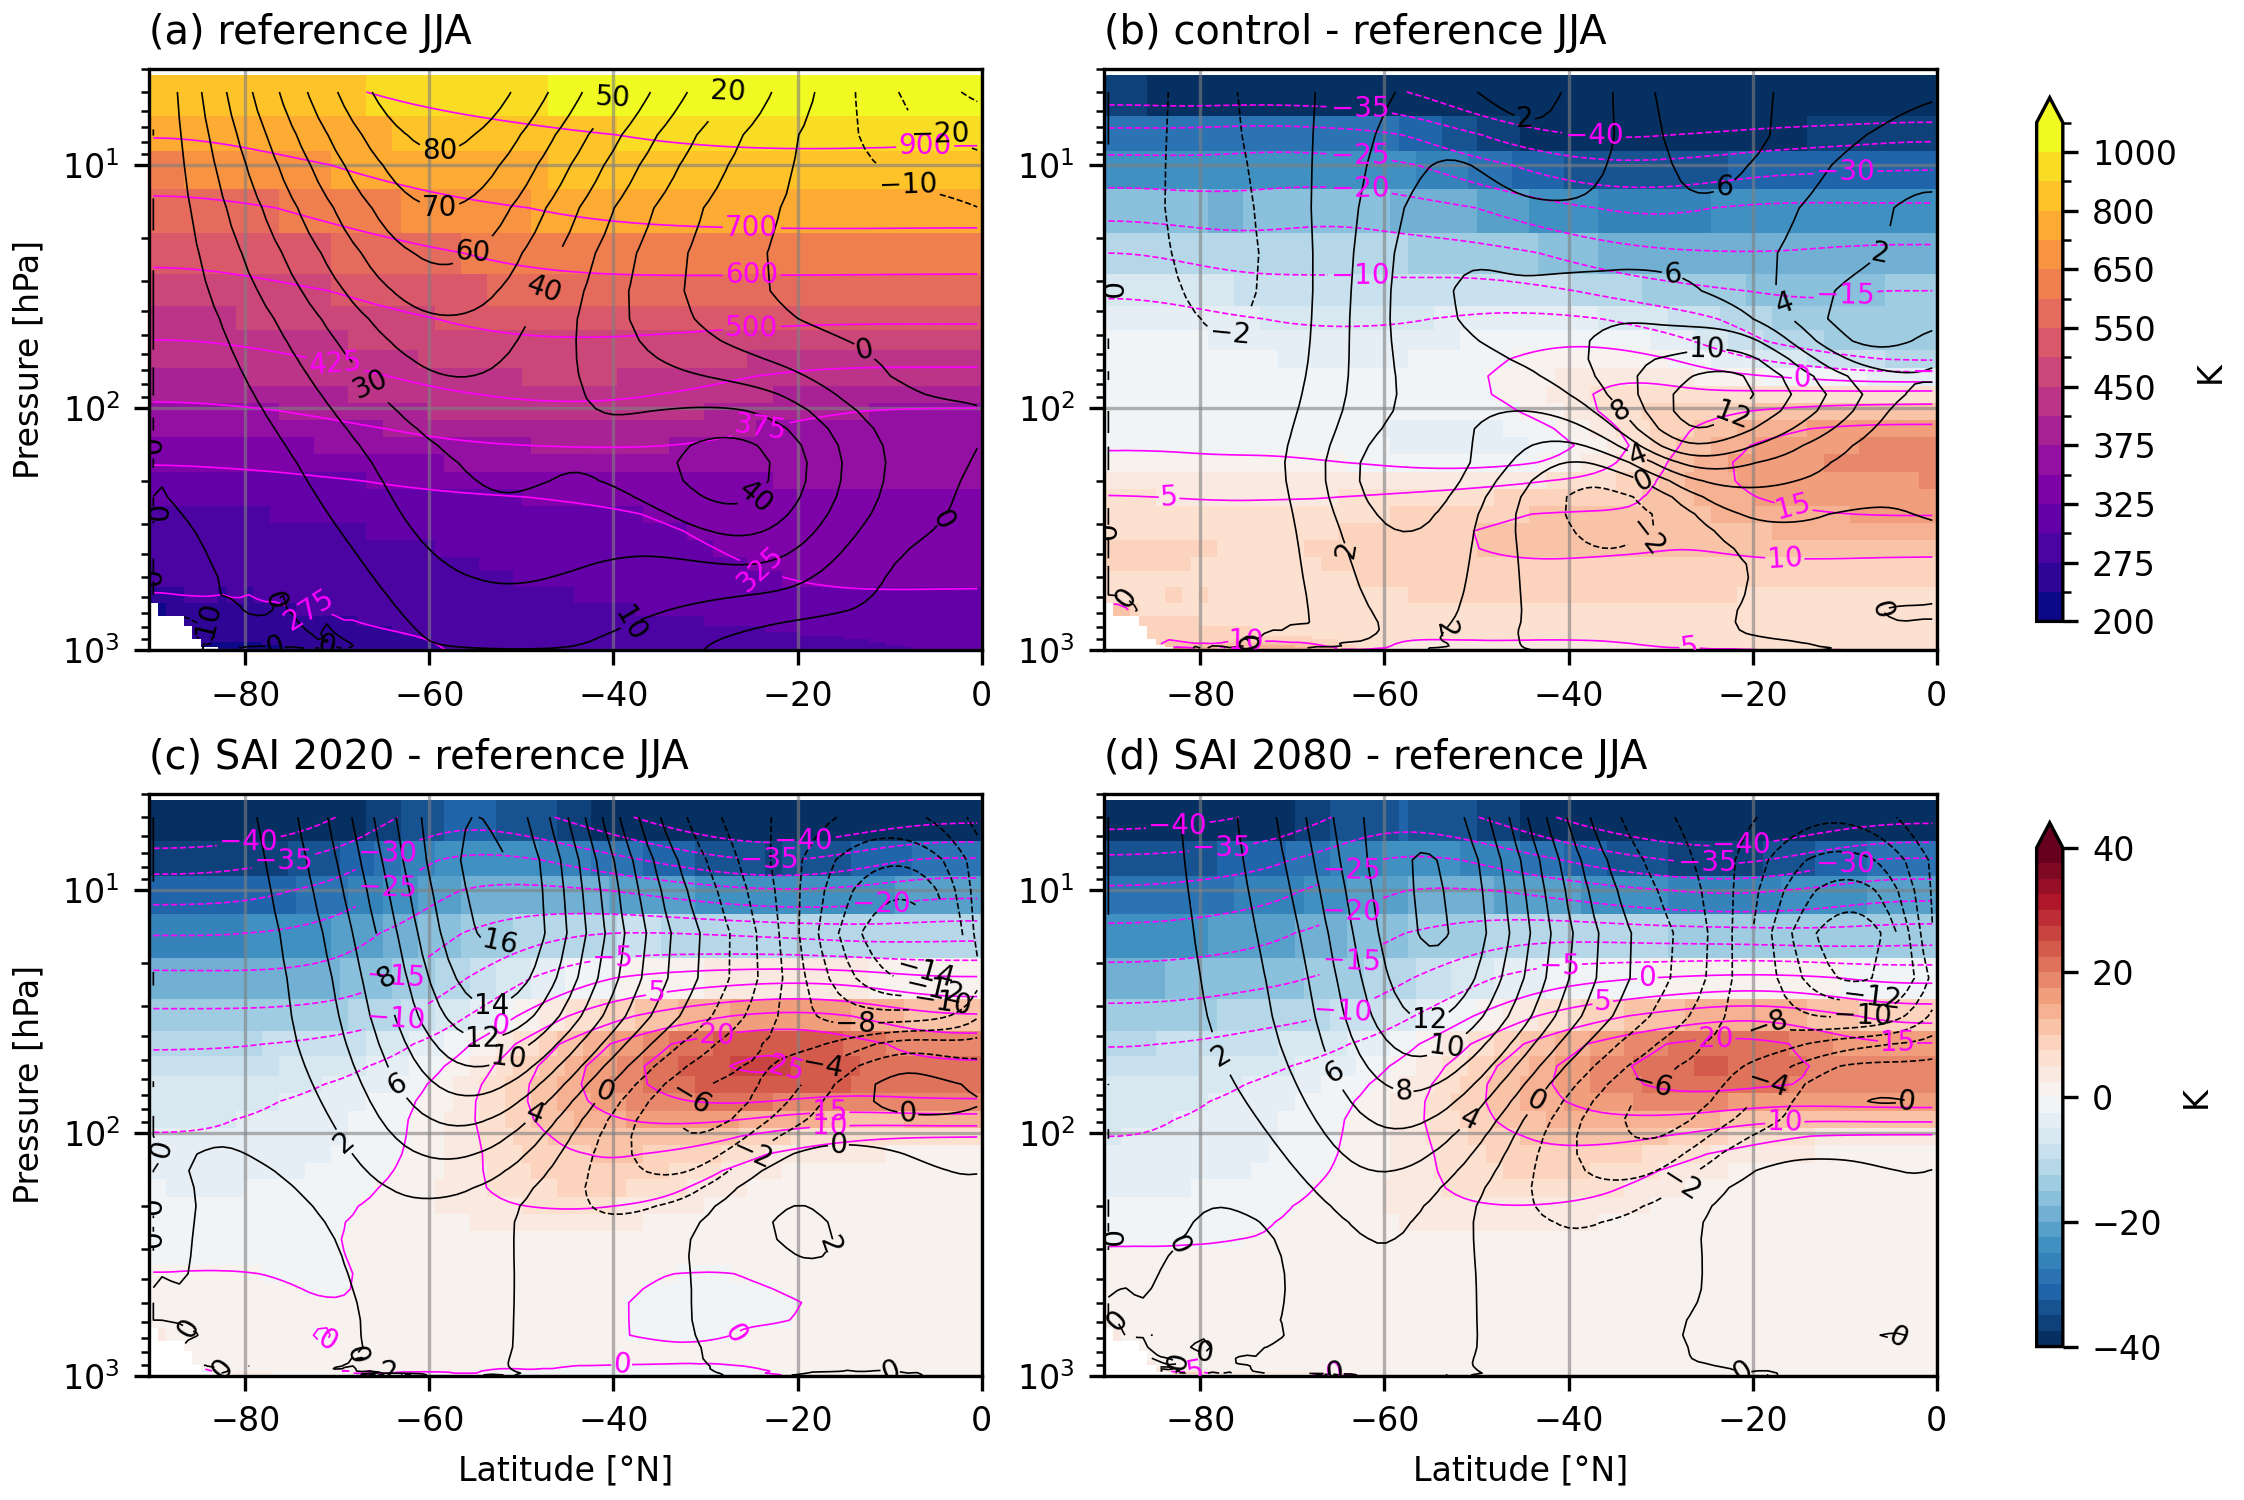
\includegraphics[width=0.95\linewidth]{images/th_U_zmdiff_JJA.png}
	\caption{JJA mean zonal mean potential temperature (shading and black contours) and zonal mean zonal wind (magenta contours) for (a): Reference; (b-d): Control, SAI 2020 and SAI 2080 anomaly compared to Reference.}
	\label{fig:th_U_zmdiff_JJA}
\end{figure}

\begin{figure}[H]
	\centering
	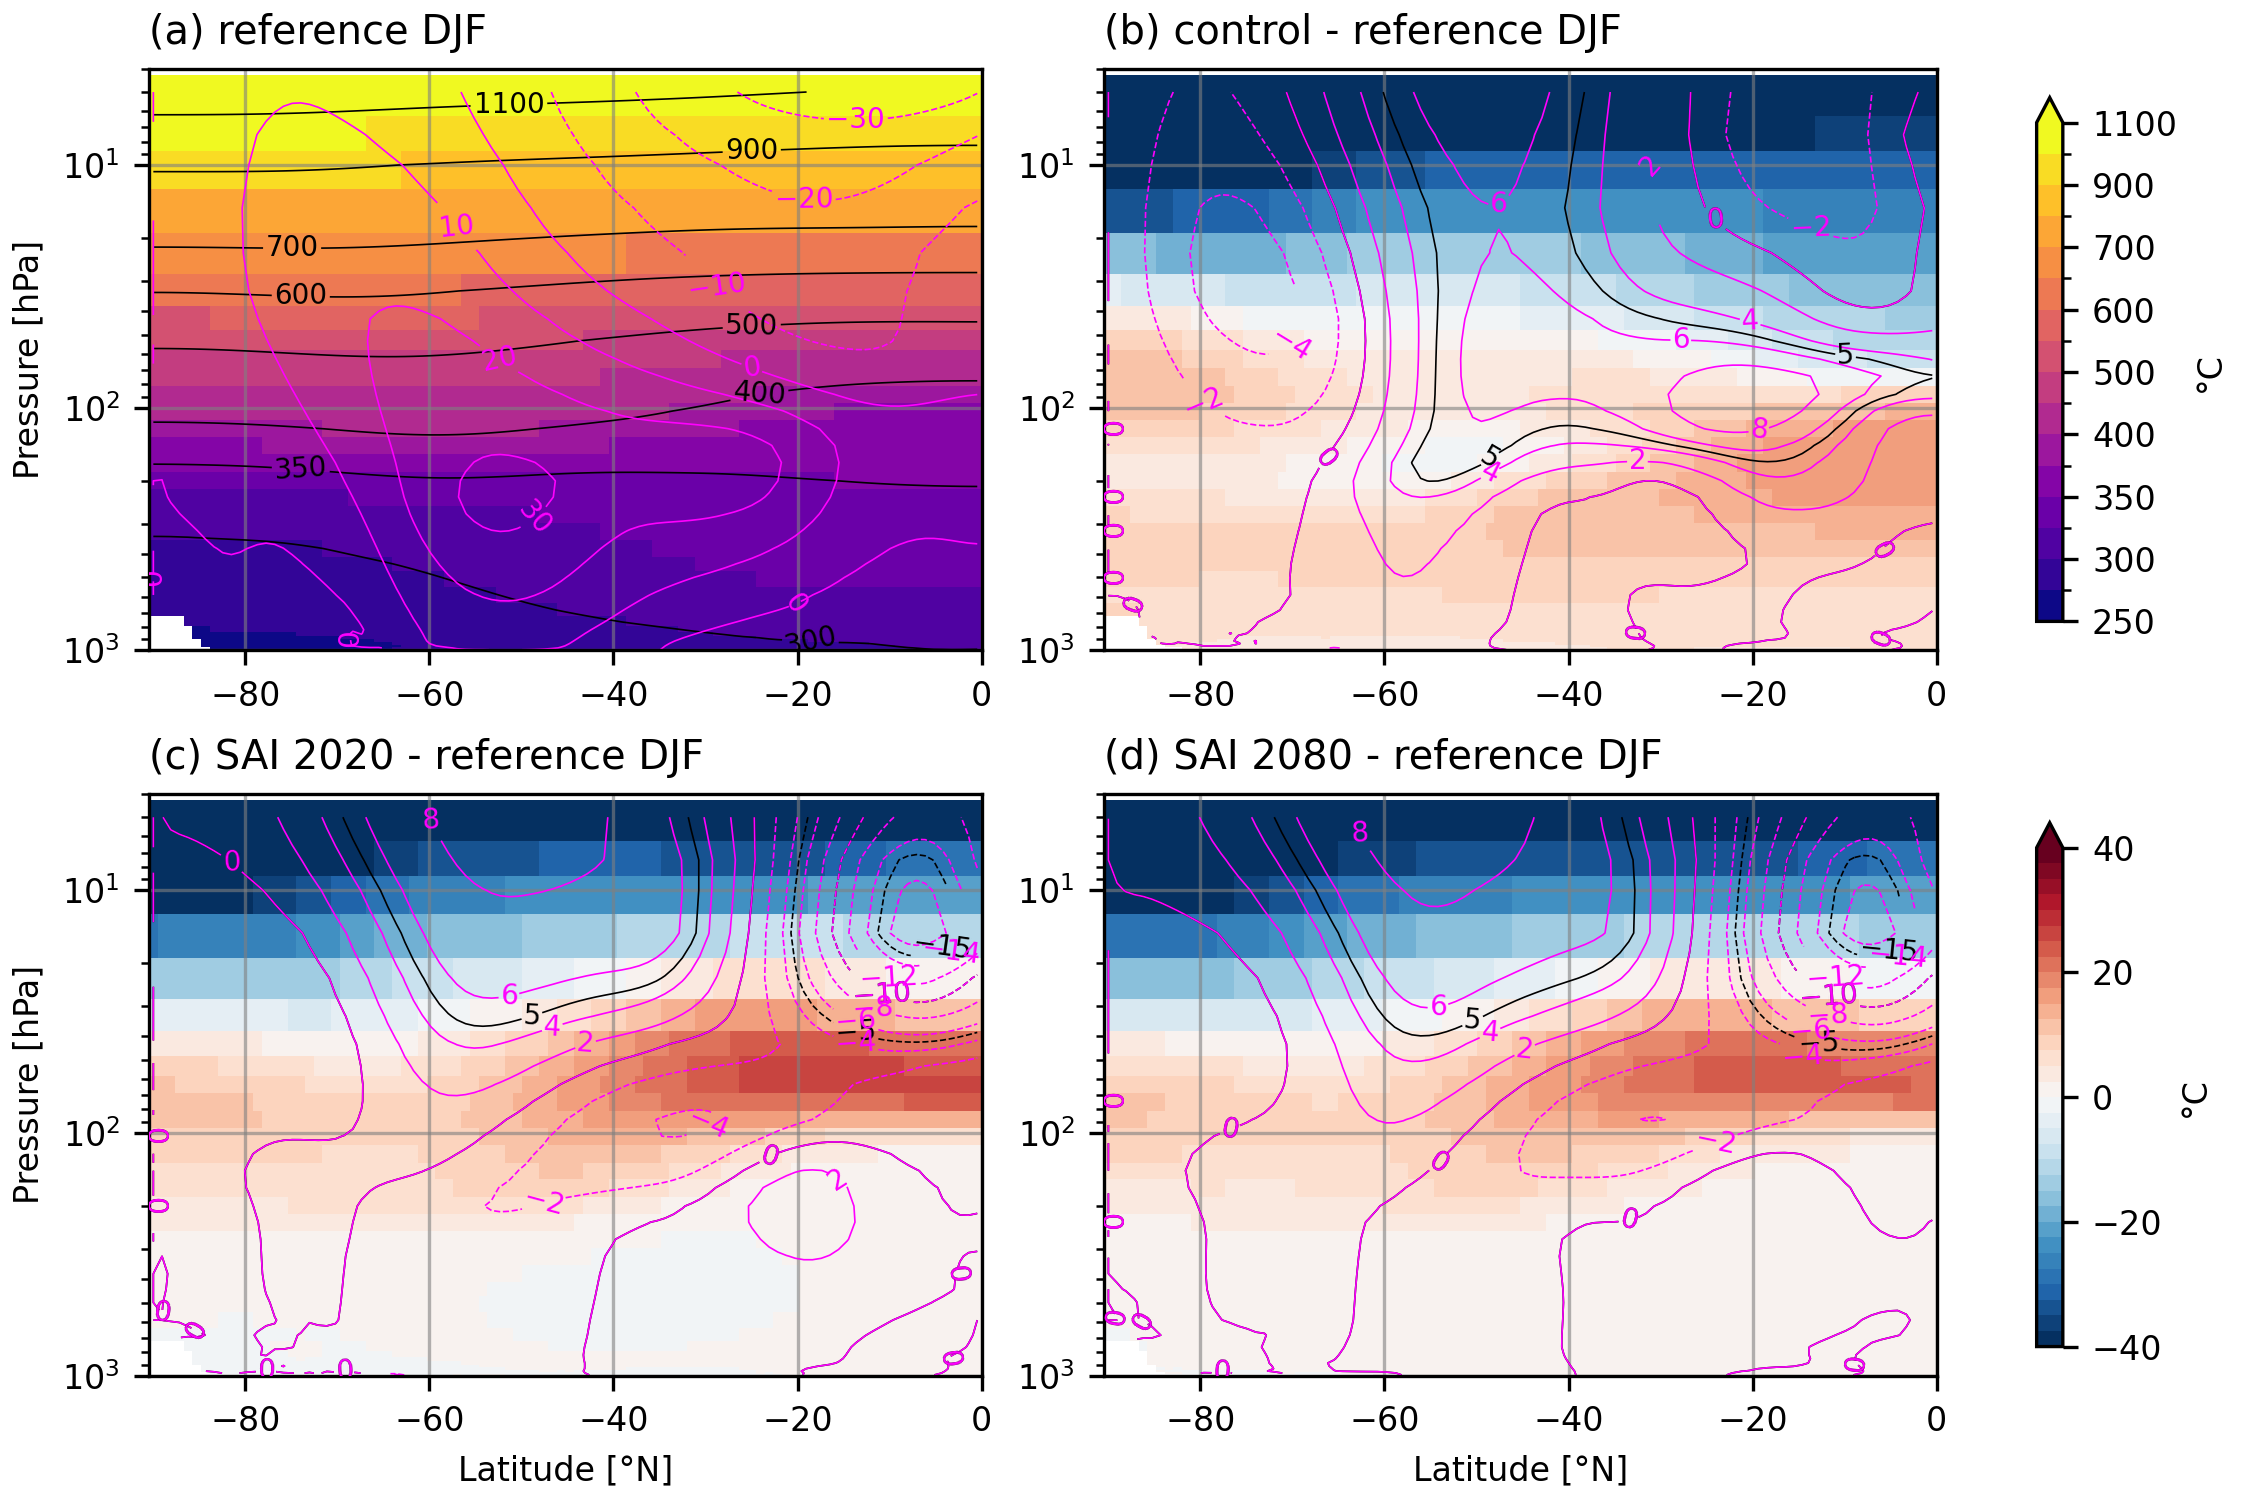
\includegraphics[width=0.95\linewidth]{images/th_U_zmdiff_DJF.png}
	\caption{DJF mean zonal mean potential temperature (shading and black contours) and zonal mean zonal wind (magenta contours) for (a): Reference; (b-d): Control, SAI 2020 and SAI 2080 anomaly compared to Reference.}
	\label{fig:th_U_zmdiff_DJF}
\end{figure}


\subsection{Subtropical Jet}
The change in magnitude of the lower stratosphere wind strongly correlates with the change in magnitude of the zonal component of the thermal wind. The subtropical jet (STJ) around 25°S and 200 hPa shifts upward and equatorwad, also showing a significant increase. In contrast, in both SAI 2020 and SAI 2080 the STJ decreases in strength, mainly in the upper regions around 100 hPa.  

On the subtropical jet intensity map in Figure \ref{fig:STJ_map_JJA} the same trends as above are observed. In Control the jet intensifies and shifts equatorward. The largest increase is observed in the easter Pacific Ocean, where in Reference the jet is relatively weak, in Control the jet is strongest in this area.

In SAI 2020 and SAI 2080 the jet is much weaker, but the spatial distribution remains largely unchanged. The jet weakens slightly more in SAI 2080 than in SAI 2020. 

% \begin{figure}[H]
% 	\centering
% 	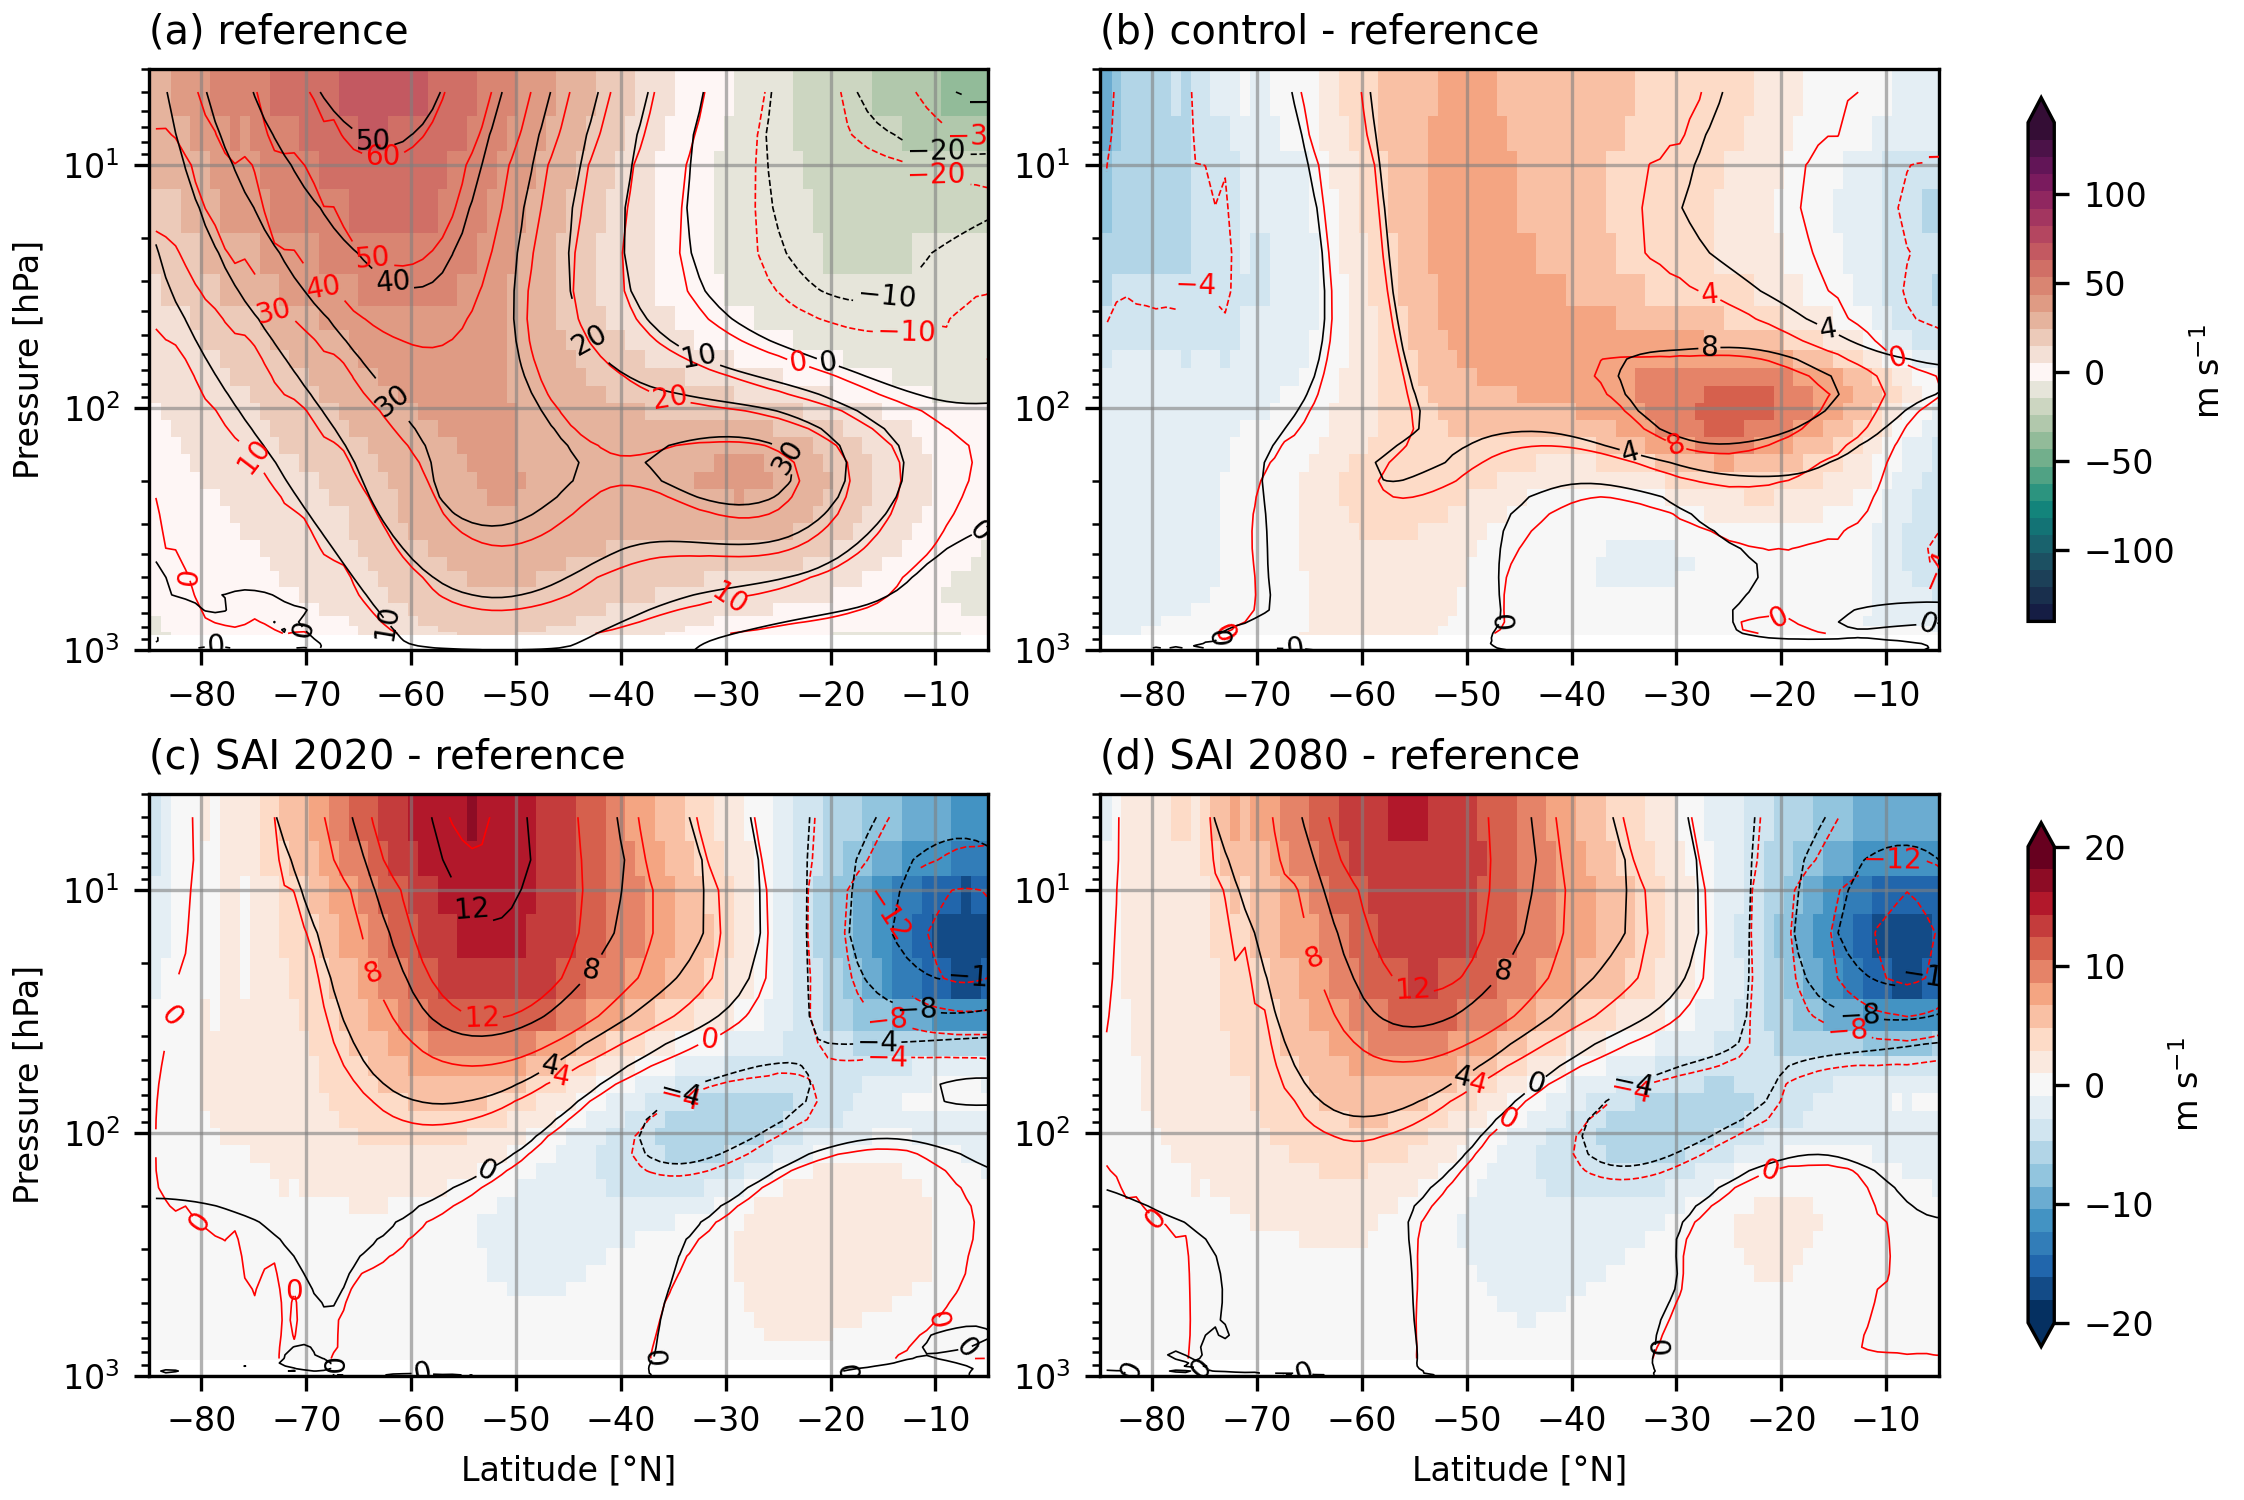
\includegraphics[width=0.95\linewidth]{images/UT_U_zmdiff_ann.png}
% 	\caption{Annual mean zonal mean zonal thermal wind (shading and black contours) and zonal mean zonal wind (red contours) for (a): Reference; (b-d): Control, SAI 2020 and SAI 2080 anomaly compared to Reference.}
% 	\label{fig:th_U_zmdiff_ann}
% \end{figure}

\begin{figure}[H]
	\centering
	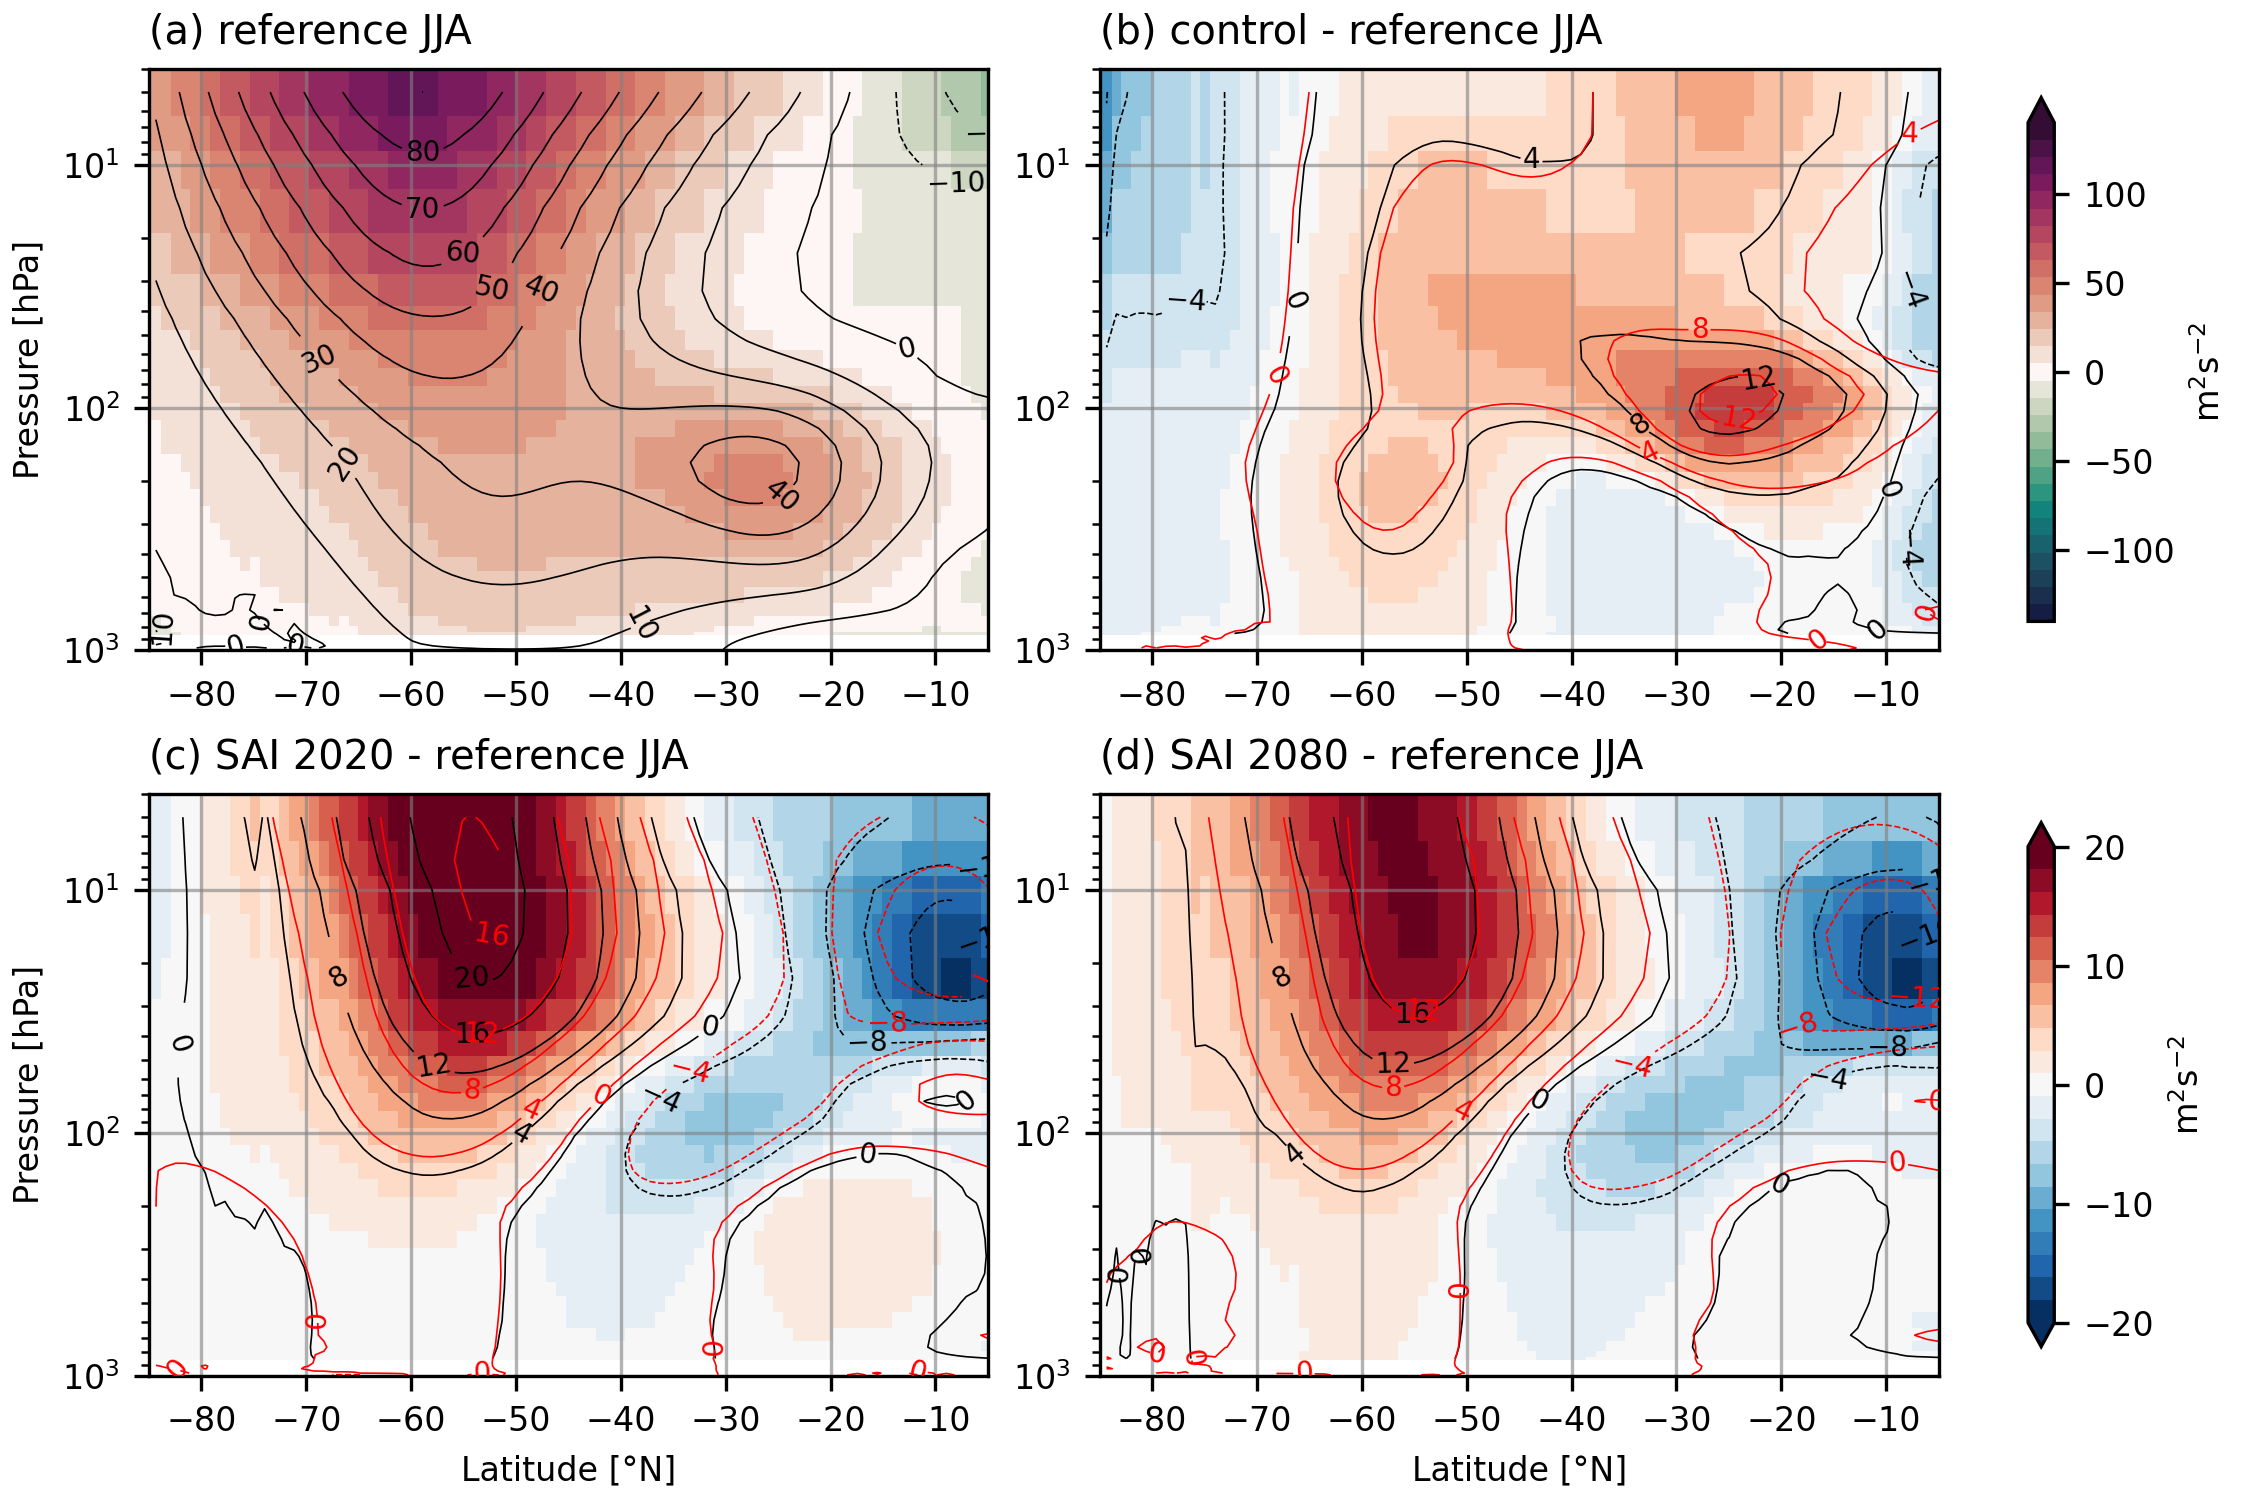
\includegraphics[width=0.95\linewidth]{images/UT_U_zmdiff_JJA.png}
	\caption{JJA mean zonal mean zonal thermal wind (shading and black contours) and zonal mean zonal wind (red contours) for (a): Reference; (b-d): Control, SAI 2020 and SAI 2080 anomaly compared to Reference.}
	\label{fig:th_U_zmdiff_JJA}
\end{figure}

% \begin{figure}[H]
% 	\centering
% 	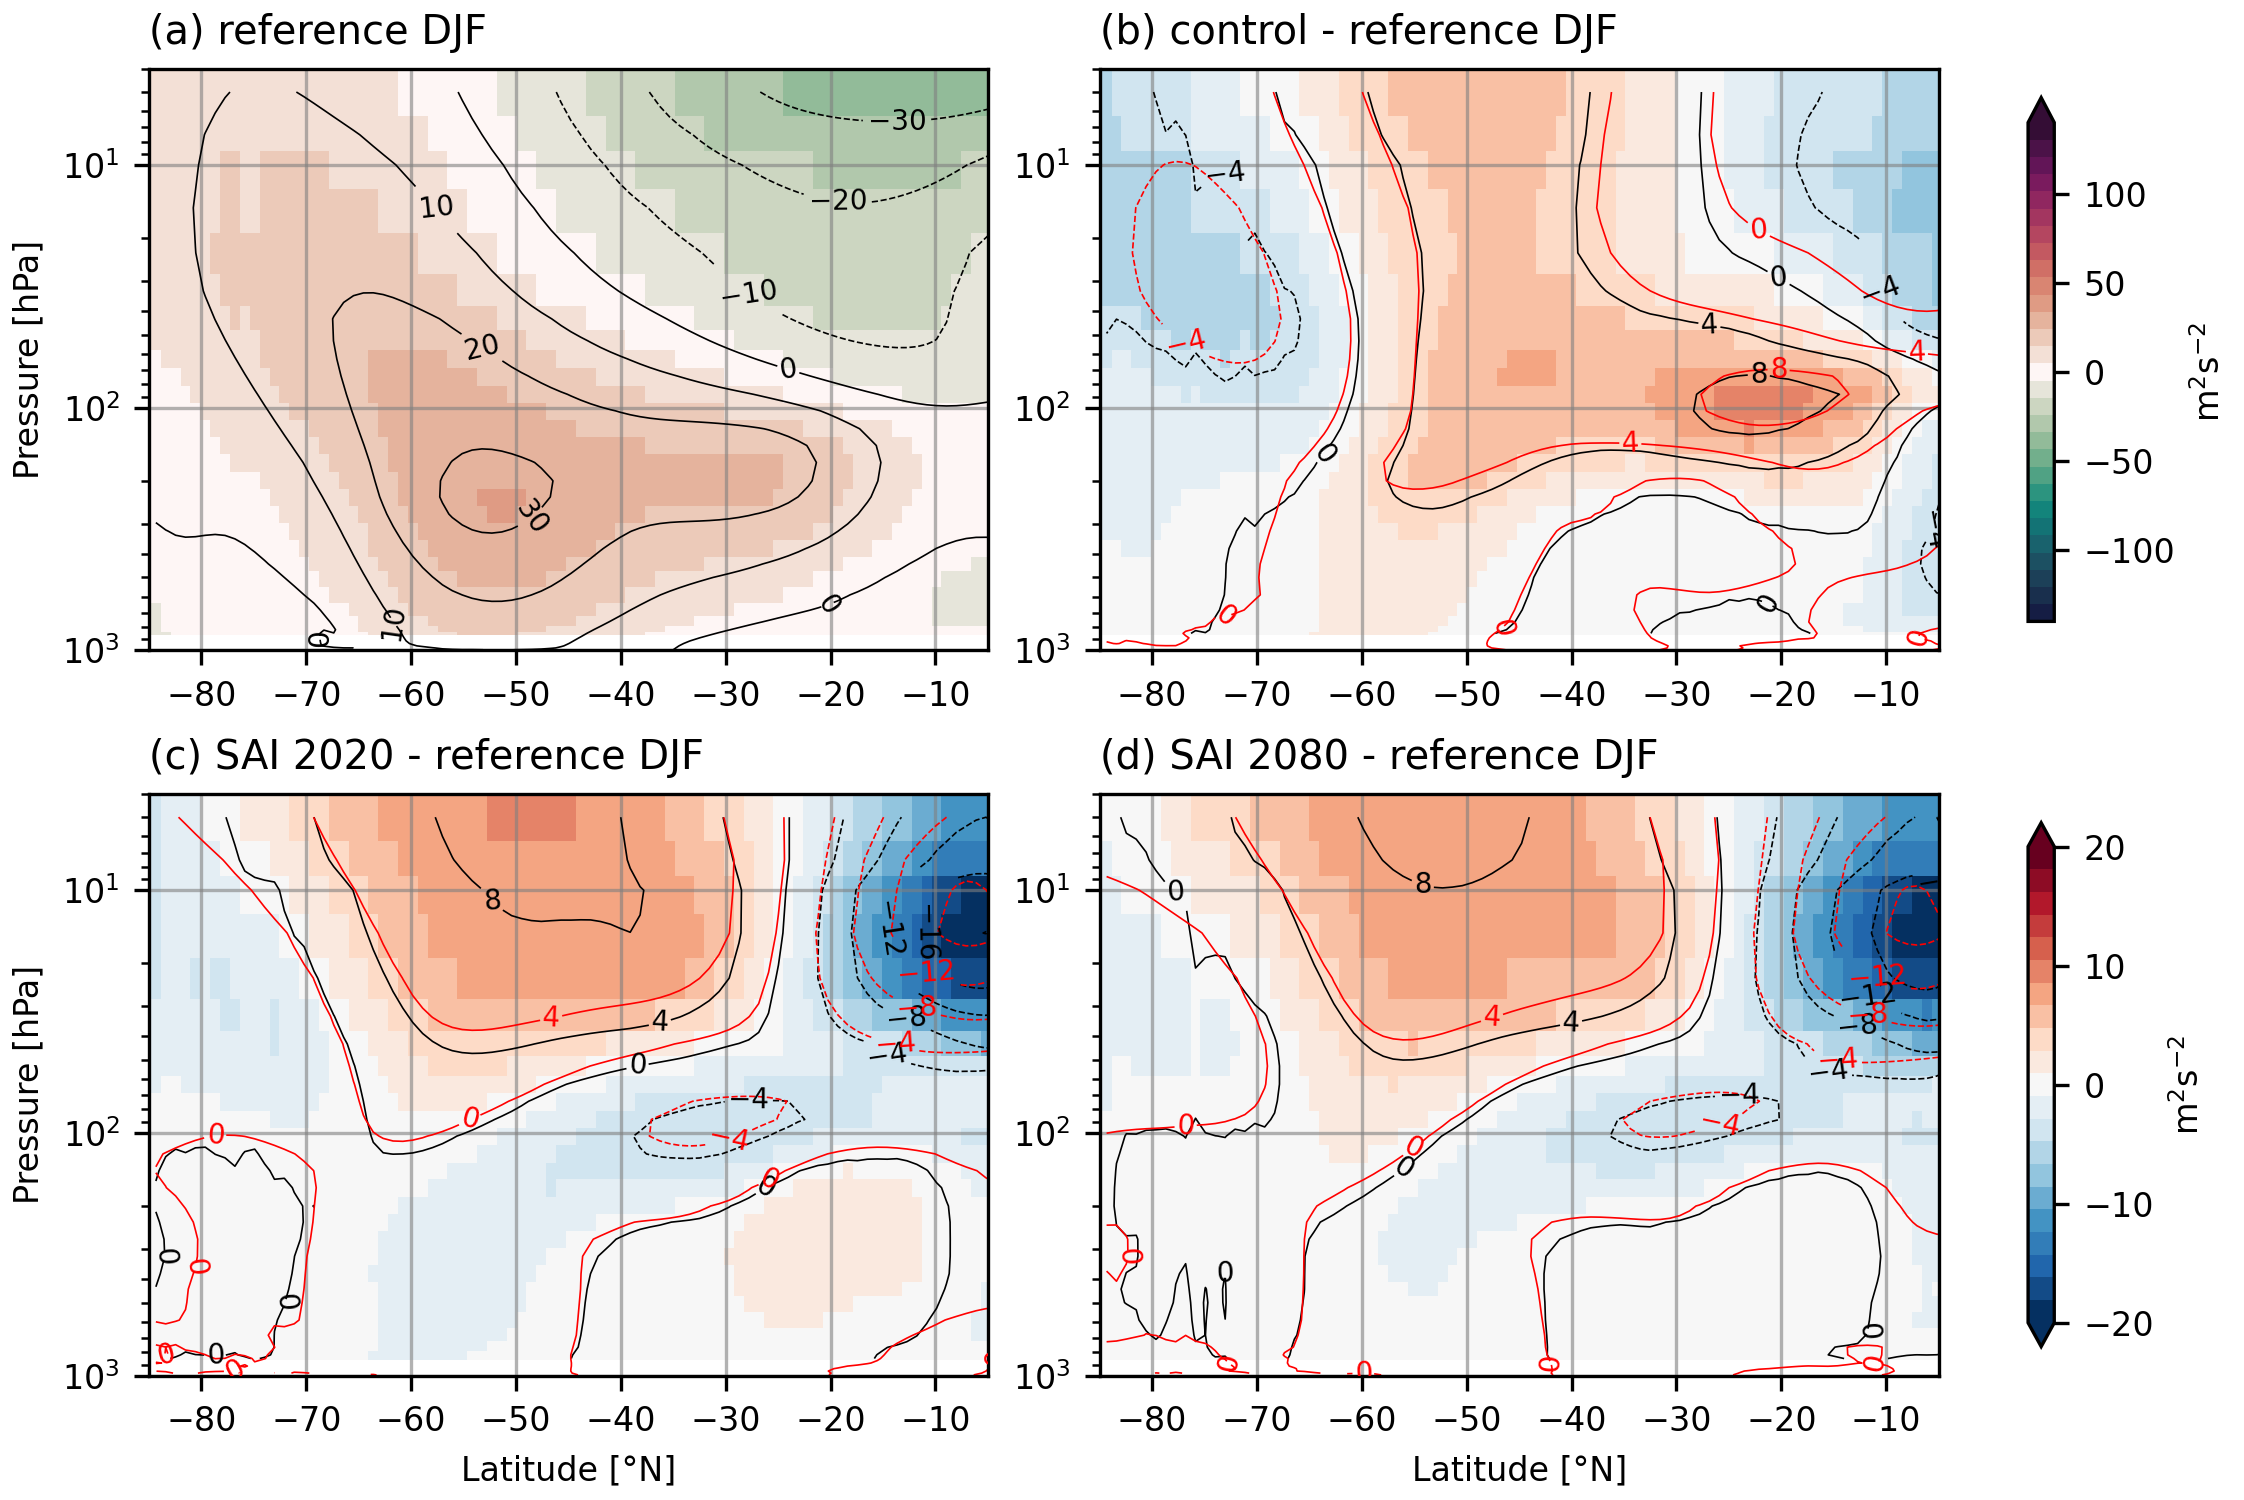
\includegraphics[width=0.95\linewidth]{images/UT_U_zmdiff_DJF.png}
% 	\caption{DJF mean zonal mean zonal thermal wind (shading and black contours) and zonal mean zonal wind (red contours) for (a): Reference; (b-d): Control, SAI 2020 and SAI 2080 anomaly compared to Reference.}
% 	\label{fig:th_U_zmdiff_DJF}
% \end{figure}

\begin{figure}[H]
	\centering
	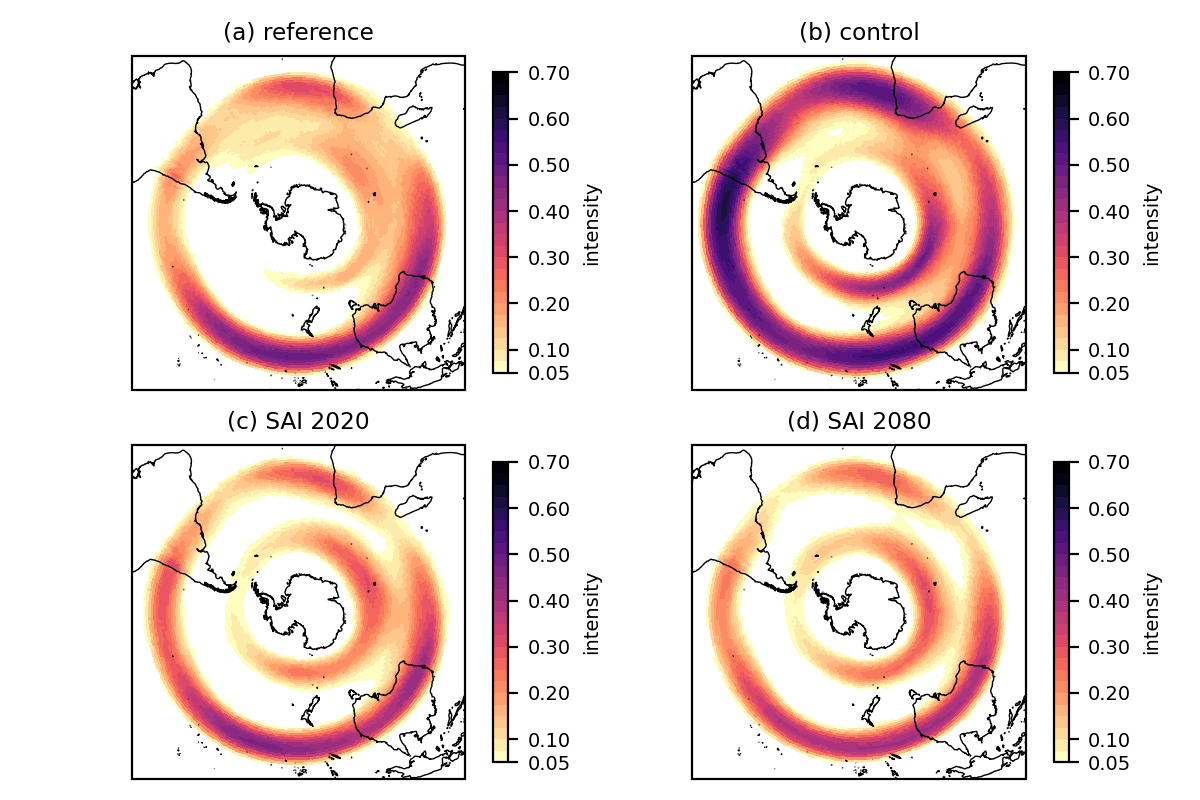
\includegraphics[width=0.95\linewidth]{images/STJ_map_JJA.png}
	\caption{JJA subtropical jet intensity map for (a) Reference, (b) Control, (c) SAI 2020 and (d) SAI 2080.}
	\label{fig:STJ_map_JJA}
\end{figure}


\subsection{Eddy-driven Jet}
More poleward, around 50°S, another jet structure appears, mostly visible in Figure \ref{fig:STJ_map_JJA}. The zonal wind in this area increases, most notably in Control, which is also visible in Figure \ref{fig:th_U_zmdiff_JJA}. Beacuse this jet is driven by eddy activity, the zonal mean eddy kinetic energy (EKE) and EKE anomalies are shown in Figure \ref{fig:EKE_U_zmdiff_JJA}.

Around 50°S and 300 hPa, there is a peak in EKE, i.e. high eddy activity. In Control the EKE decreases on the lower equatorward side of the jet and increases on the upper poleward side, indicating that the jet shifts poleward and upward. In SAI 2020 and SAI 2080 the EKE shows small changes relative to Control, with the most notable change the decrease around 45°S, right in between the EDJ and the STJ. 

The eddy-driven jet intensity map in Figure \ref{fig:EDJ_map_JJA} is also shown to increase in intensity in Control and slightly decrease in both SAI 2020 and SAI 2080. The spatial pattern remains largely unchanged in all scenarios. 

\begin{figure}[H]
	\centering
	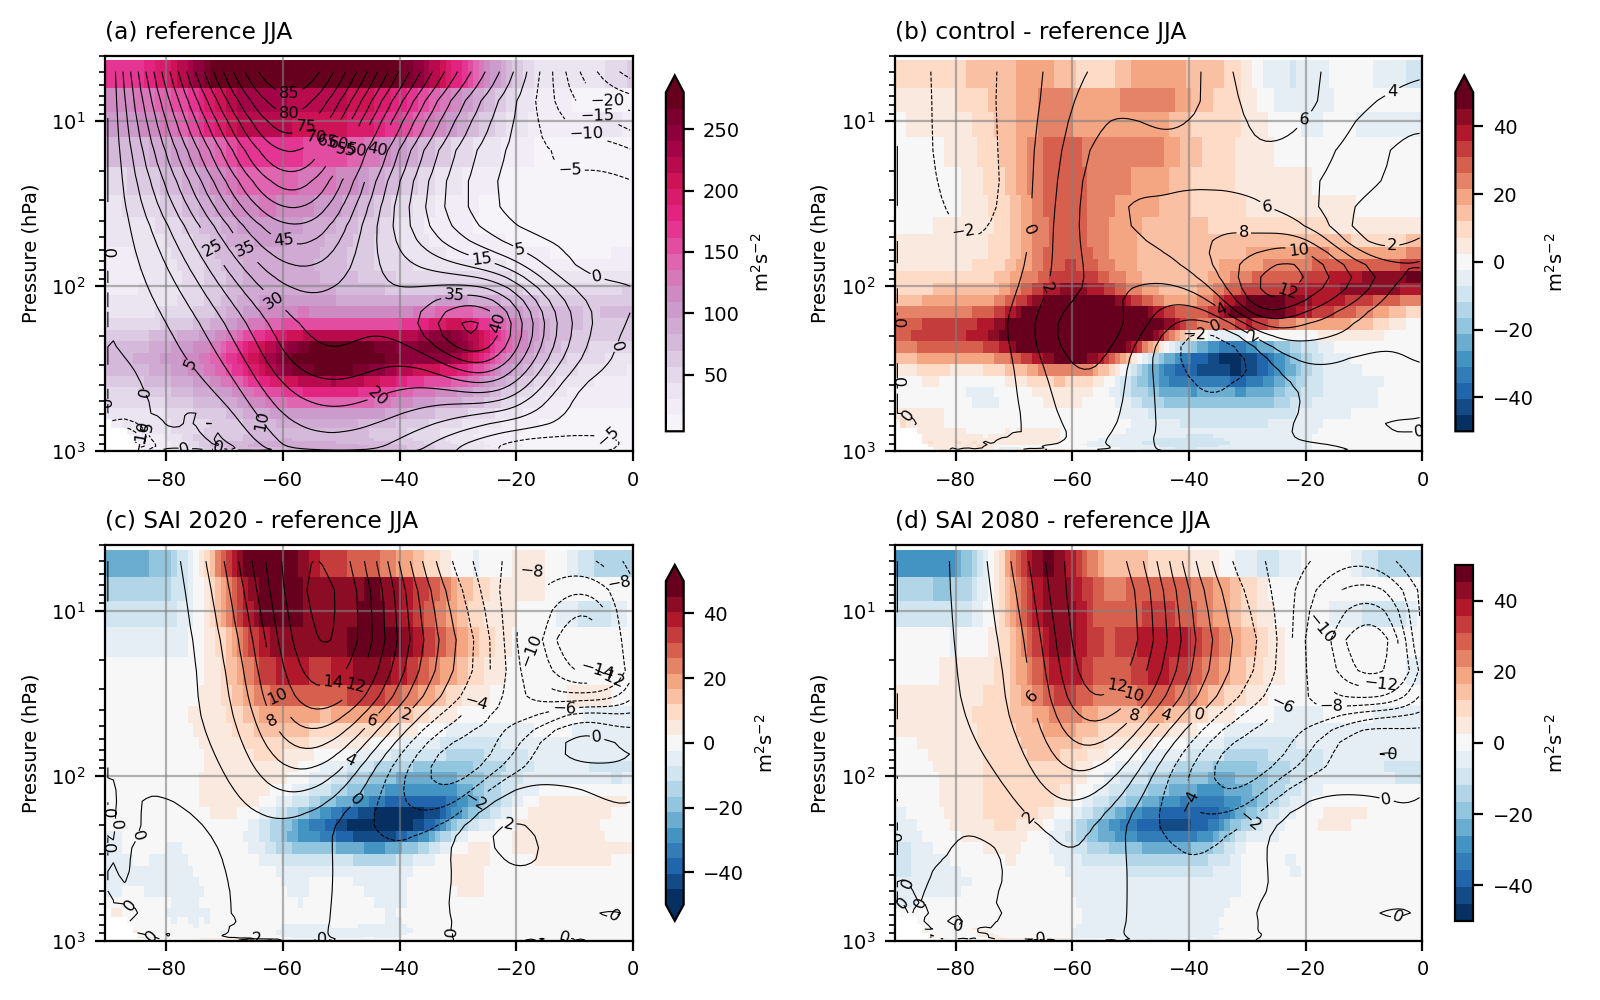
\includegraphics[width=0.95\linewidth]{images/EKE_U_zmdiff_JJA.png}
	\caption{JJA mean zonal mean eddy kinetic energy (shading) and zonal mean zonal wind (contours) for (a): Reference; (b-d): Control, SAI 2020 and SAI 2080 anomaly compared to Reference.}
	\label{fig:EKE_U_zmdiff_JJA}
\end{figure}

\begin{figure}[H]
	\centering
	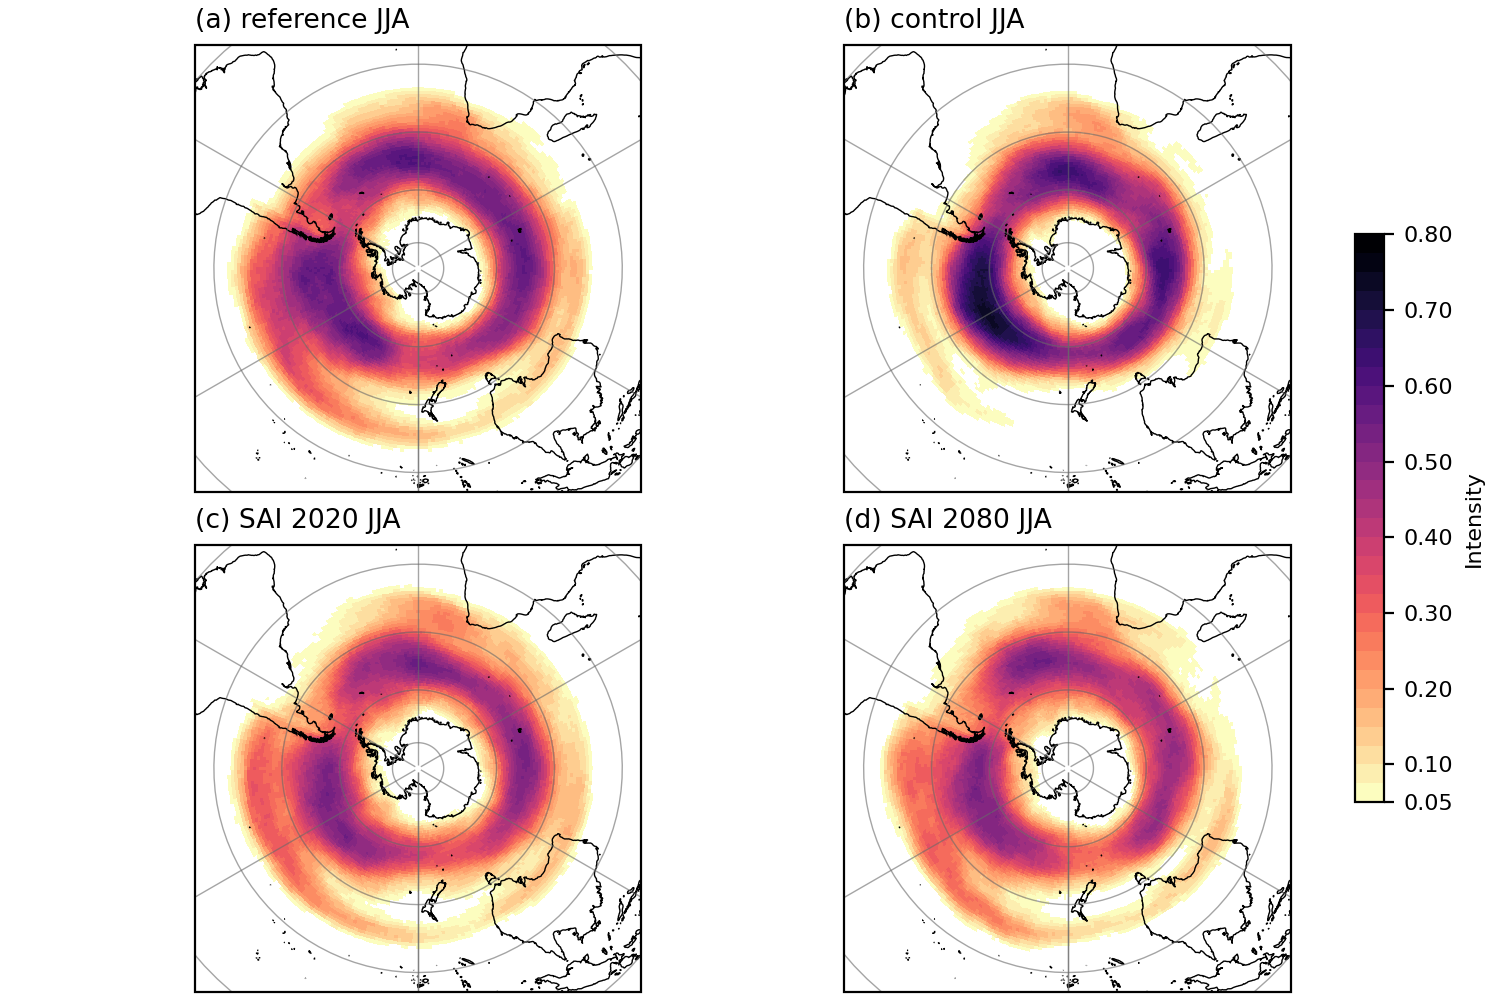
\includegraphics[width=0.95\linewidth]{images/EDJ_map_JJA.png}
	\caption{JJA eddy-driven jet intensity map for (a) Reference, (b) Control, (c) SAI 2020 and (d) SAI 2080.}
	\label{fig:EDJ_map_JJA}
\end{figure}

There is a clear correlation between the EKE anomalies and zonal mean zonal wind anomalies, thus we look at the kinetic energy to disentangle the change in zonal wind from the change in EKE. In Figure \ref{fig:KE_U_zmdiff_JJA} the zonal mean kinetic energy and zonal mean zonal wind are shown. 

For Control the increase in KE energy follows the zonal wind patterns in sign, but not in magnitude. The KE increases with the increasing zonal wind accordingly in the upper regions of the STJ, but the KE increases and decreases more in the EDJ area than would be expedted from the increase in zonal wind. \textcolor{teal}{Sidenote: de plot voor KE is niet goed, de extents van de colormap gaan niet ver genoeg dus ik kan niet heel goed zien wat er nou gebeurt in control, voor nu hou ik het hierbij.}

For SAI 2020 and SAI 2080 the KE anomaly does follow the zonal wind anomaly proportionally and comparison with Figure \ref{fig:EKE_U_zmdiff_JJA} shows that the decrease in EKE is correlated with the decrease in zonal wind. This correlation is also clear when comparing the jet intensity maps in Figures \ref{fig:SJT_map_JJA} and \ref{fig:EDJ_map_JJA}.

\begin{figure}[H]
	\centering
	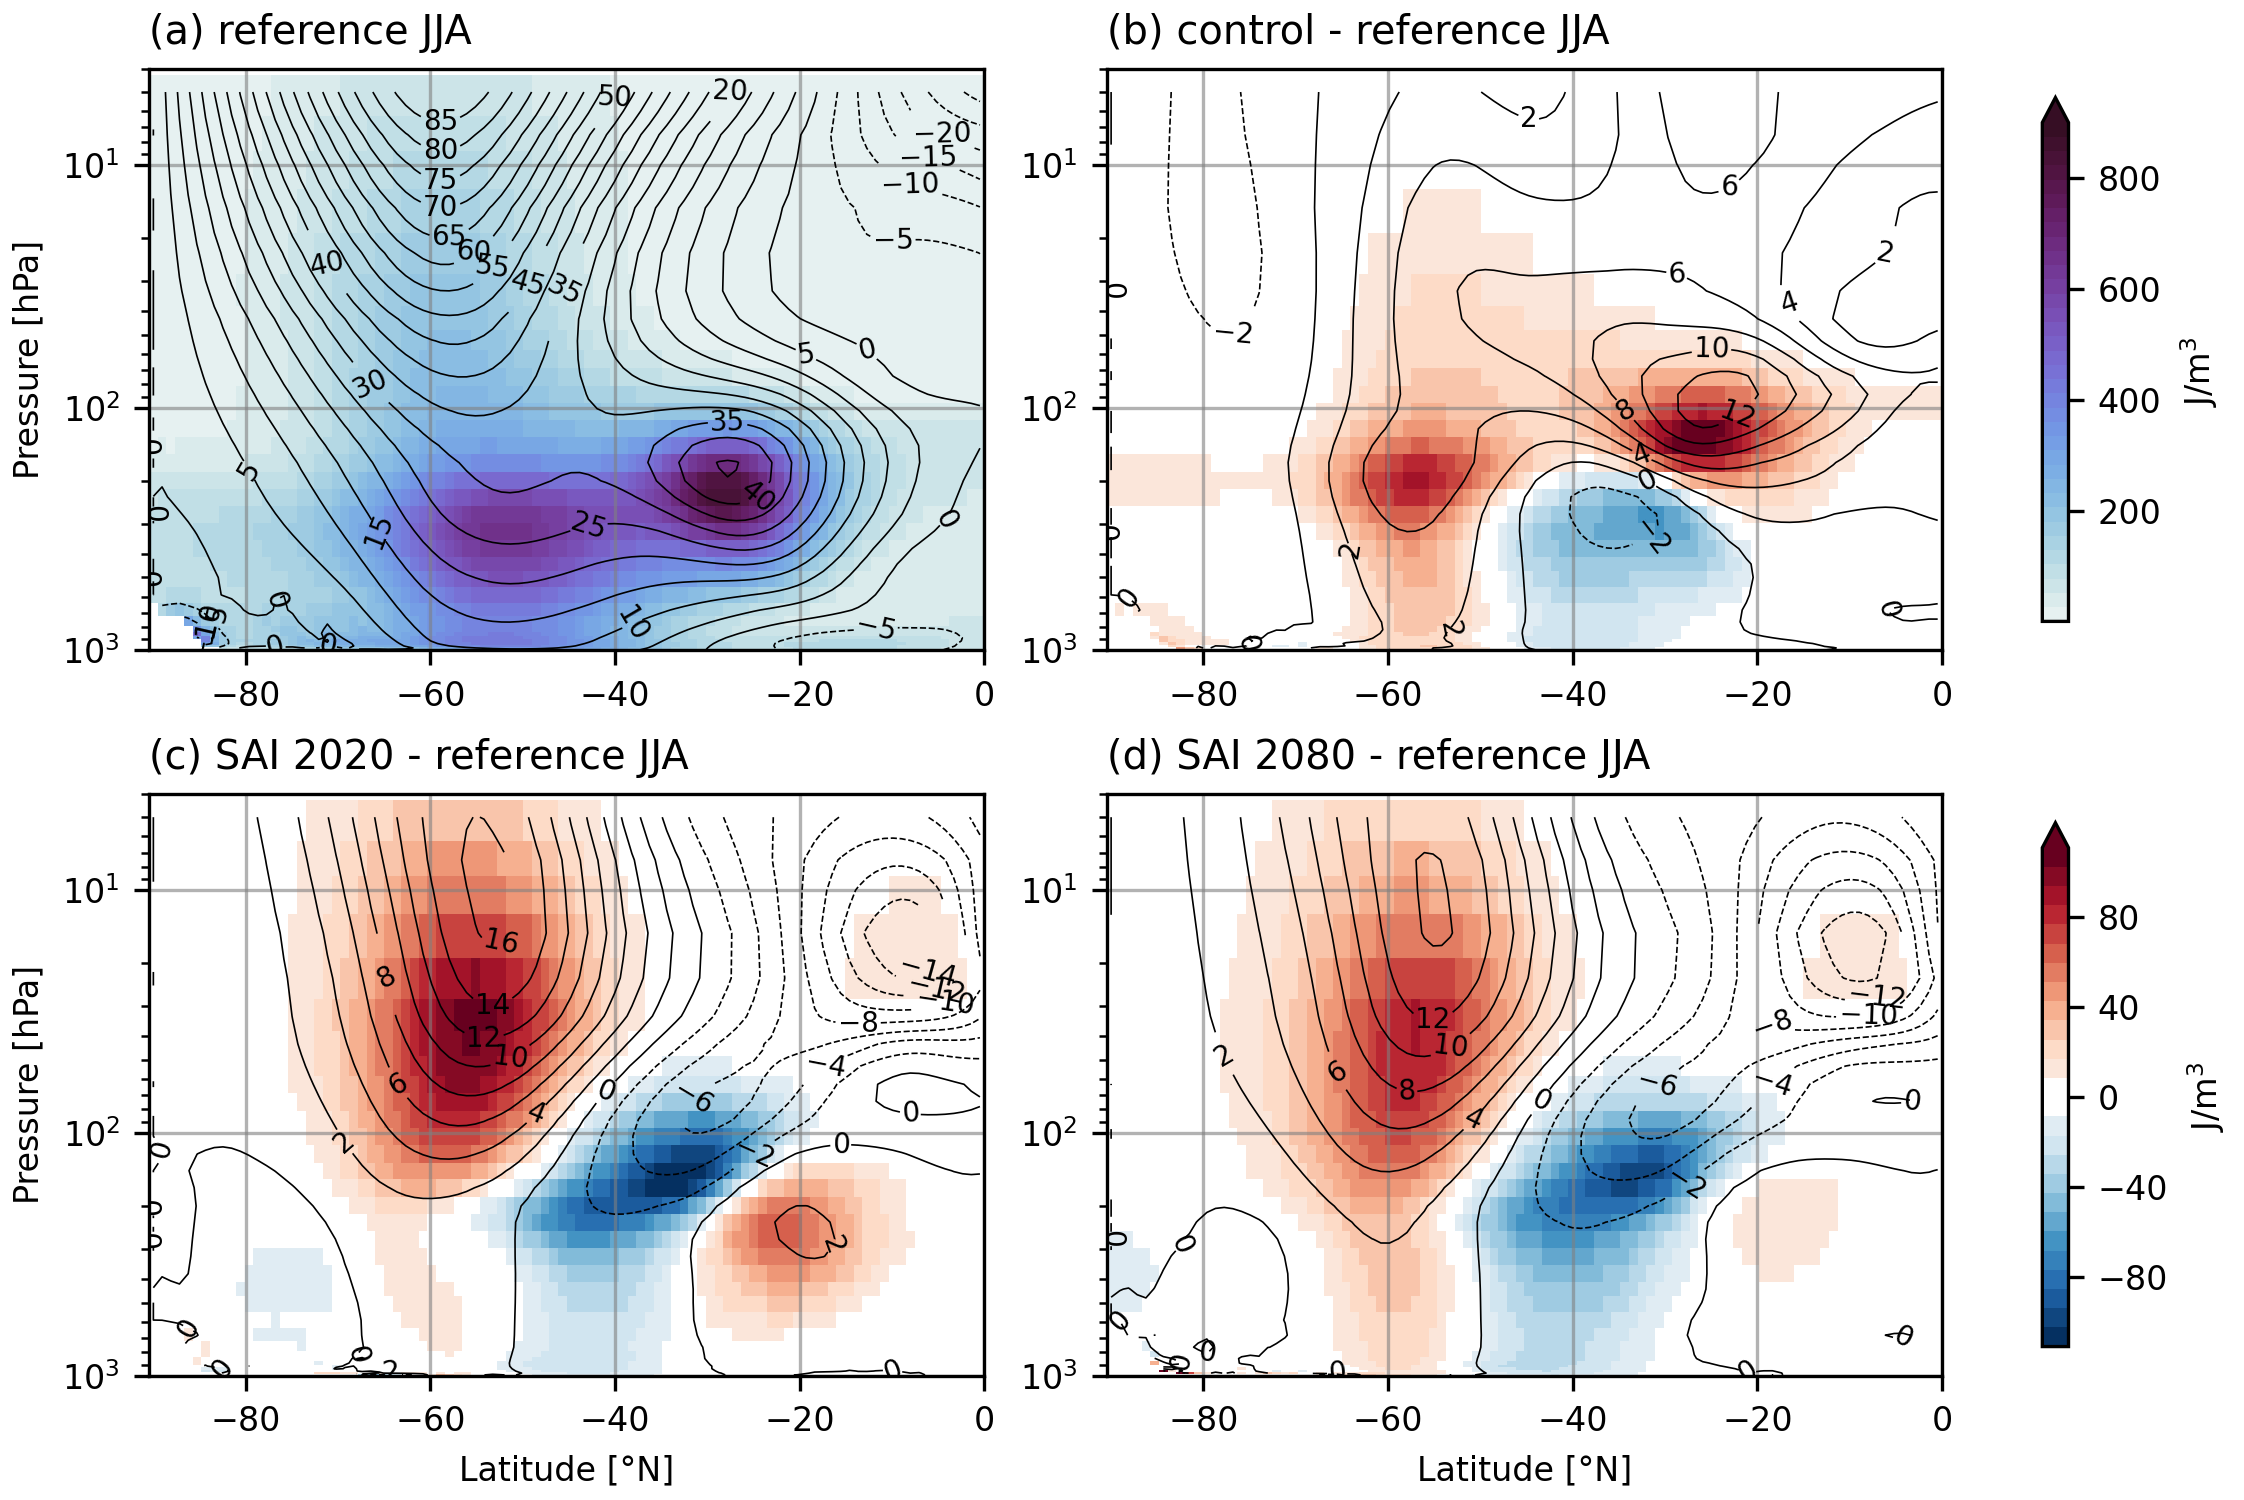
\includegraphics[width=0.95\linewidth]{images/KE_U_zmdiff_JJA.png}
	\caption{JJA mean zonal mean kinetic energy (shading) and zonal mean zonal wind (contours) for (a): Reference; (b-d): Control, SAI 2020 and SAI 2080 anomaly compared to Reference.}
	\label{fig:KE_U_zmdiff_JJA}
\end{figure}